%%%%%%%%%%

Two multivariate techniques are used for discriminating signal from the background being originated from $t\bar t$+jets. Both discriminants are studied in detail and performance of each of these found to be quite satisfactory. The expected exclusion limits for all assumed Higgs Boson mass in the range of [400,1000] was found to be remarkably better with the GNN discriminant for both lepton decay channels, resulting in better analysis sensitivity. 
The following plots show comparison of BDT and GNN sensitivity.

\begin{figure}[htbp!]
        
        \begin{subfigure}{\textwidth}                                                                                                                                     
        \begin{center} \setlength{\tabcolsep}{2.5pt}\footnotesize
        \begin{tabular}{c}
        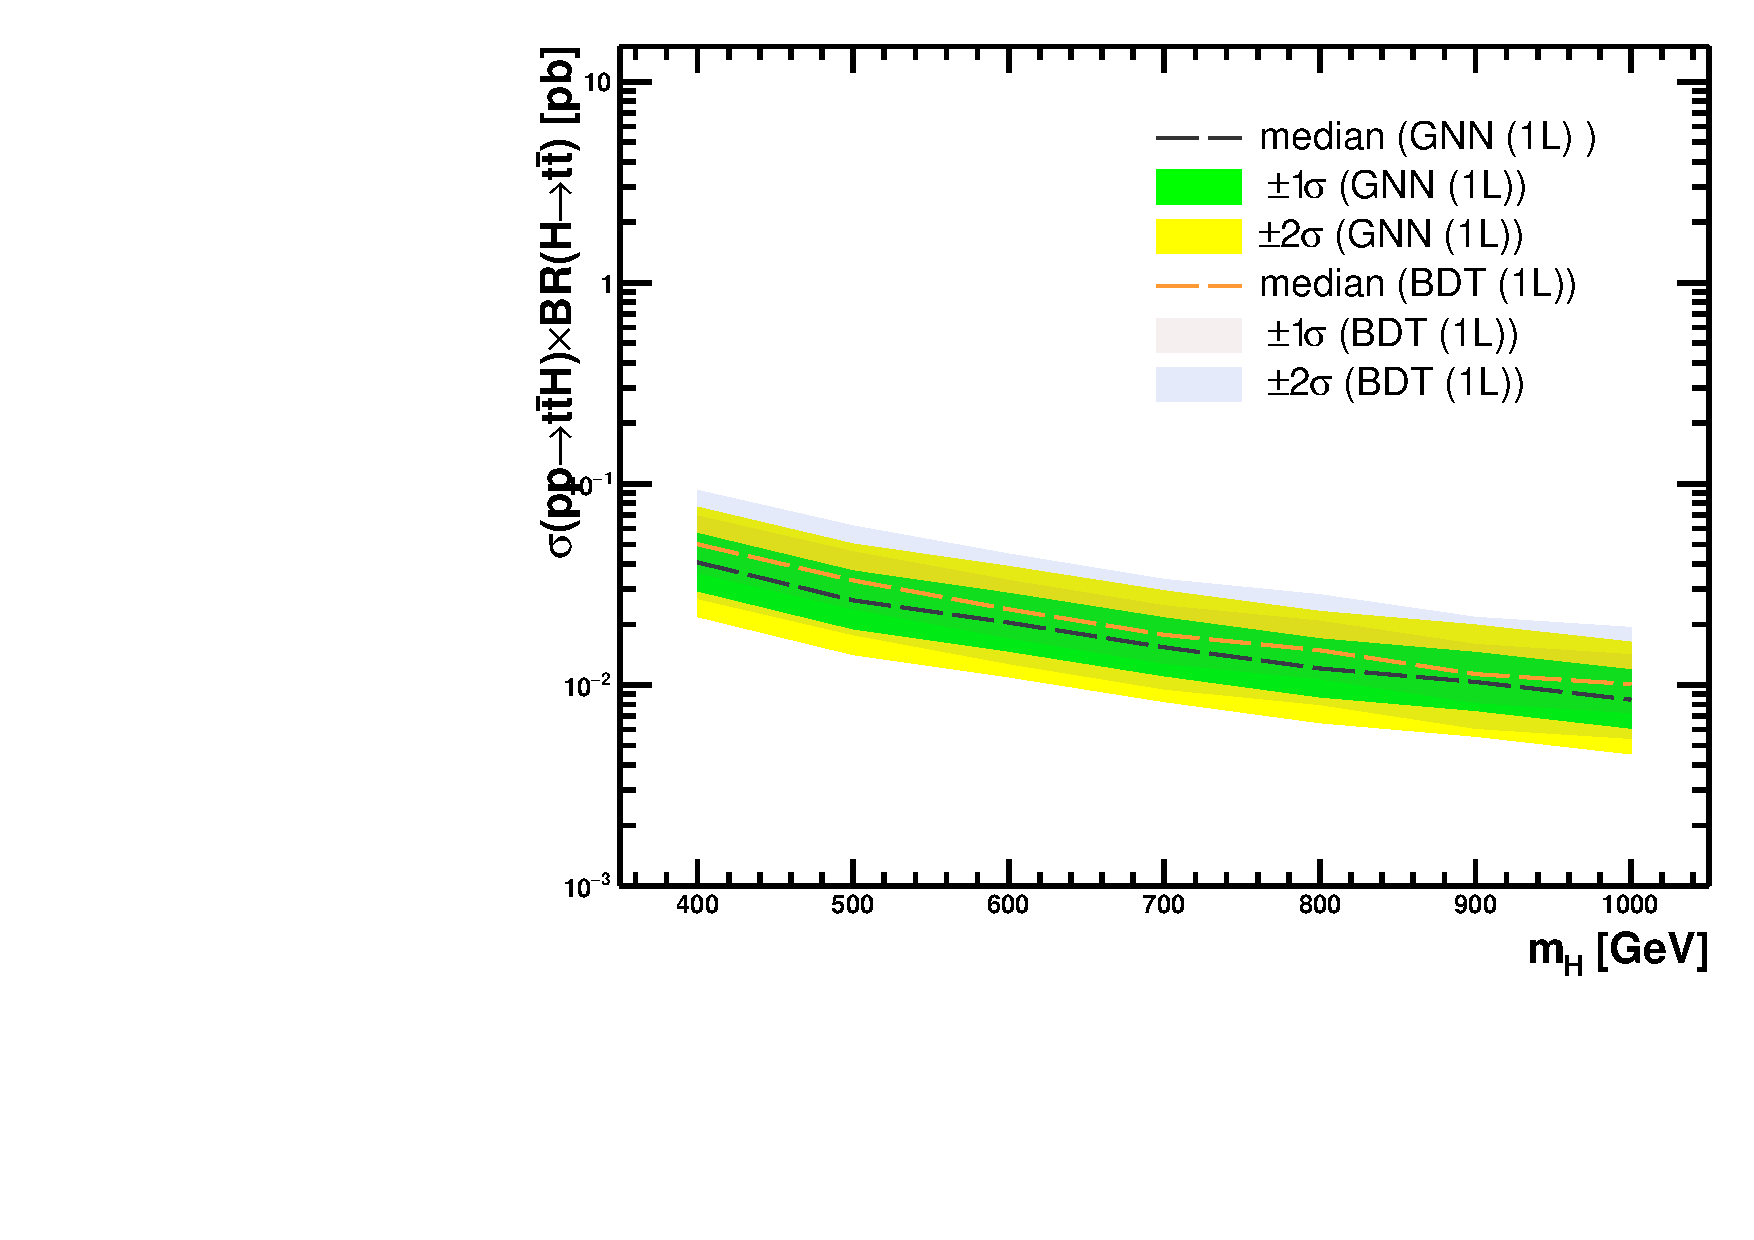
\includegraphics[width=0.45 \textwidth]{figures/limits/1L_GNNvsBDT.pdf}
        \end{tabular}
        \end{center}  
        \caption{\label{fig1:BDTvsGNN}The plot shows expected exclusion limits for all masspoints using BDT and GNN discriminant for 1L.}
        \end{subfigure}  

        \bigskip

        \begin{subfigure}{\textwidth}                                                                                                                                     
        \begin{center} \setlength{\tabcolsep}{2.5pt}\footnotesize                                                                                                         
        \begin{tabular}{c}                                                                                                                                              
        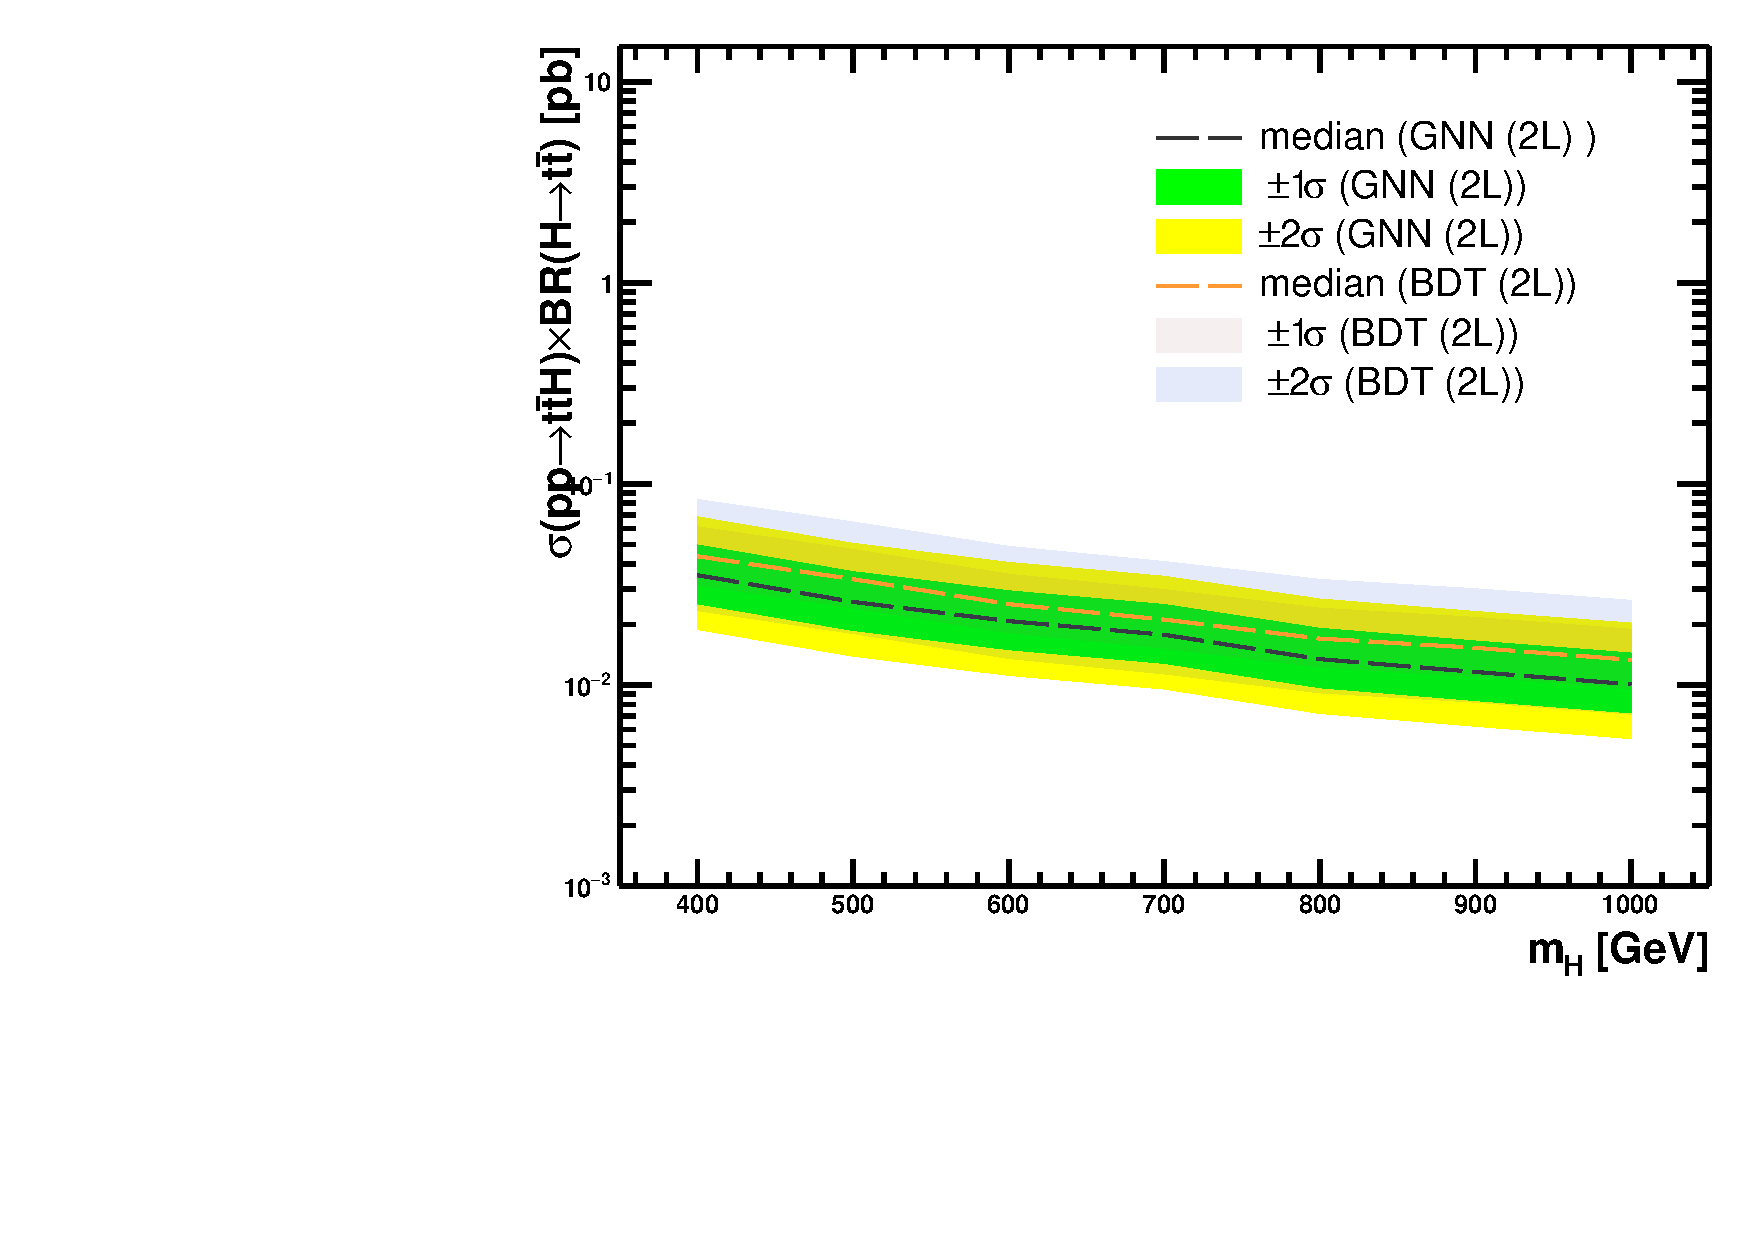
\includegraphics[width=0.45 \textwidth]{figures/limits/2L_GNNvsBDT.pdf}                                                                           
        \end{tabular}                                                                                                                                                   
        \end{center}                                                                                                                                                      
        \caption{\label{fig2:BDTvsGNN}The plot shows expected exclusion limits for all masspoints using BDT and GNN discriminant for 2L.}   
        \end{subfigure}                                                                                                                                                  
 
        \bigskip 


        \begin{subfigure}{\textwidth}                                                                                                                                     
        \begin{center} \setlength{\tabcolsep}{2.5pt}\footnotesize                                                                                                         
        \begin{tabular}{c}                                                                                                                                               
        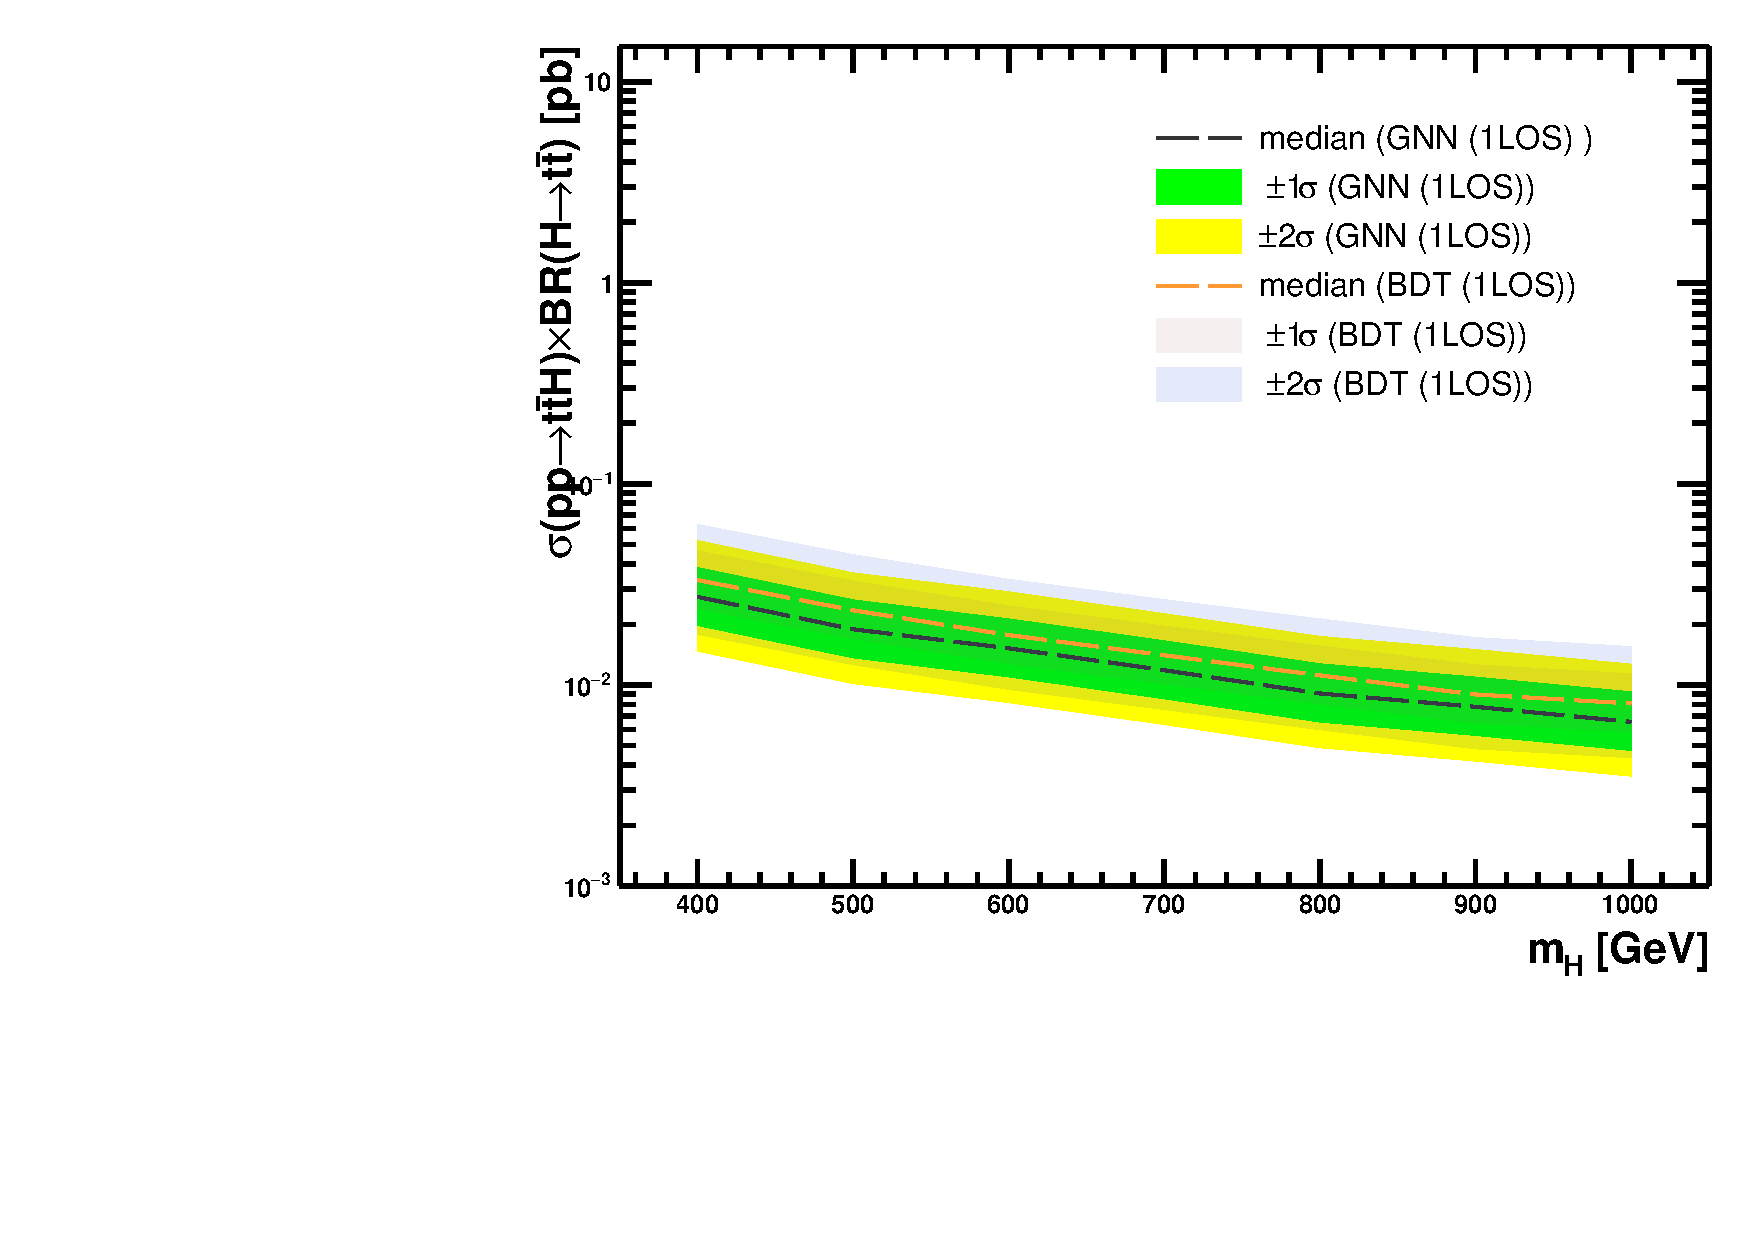
\includegraphics[width=0.45 \textwidth]{figures/limits/all_GNNvsBDT.pdf}                                                                         
        \end{tabular}                                                                                                                                                    
        \end{center}                                                                                                                                                     
        \caption{\label{fig3:BDTvsGNN}The plot shows expected exclusion limits for all masspoints using BDT and GNN discriminant for combined channel(1L+2LOS).}  
        \end{subfigure}                                                                                                                                                   
                            
        \caption{\label{BDTvsGNN}The comparison of GNN and BDT is shown in above three plots which shows GNN has better sensitivity than BDT.}                                                                                                                                              
  
\end{figure}



